%======================================================%
% Perimeter Scholars International Essay Template 2024 %
% Author: Agata Branczyk, January 2019                 %
% Last updated: 16 January 2024 by Giuseppe Sellaroli %
%======================================================%

\documentclass[12pt,twoside]{book}

%%%%%%%%%%%%%%%%%%%%%%%%%%%%%%%%%%%%%%%%%%%%%%%%%%%%%%%%%%%%%
%% EDIT THE FILE BELOW TO REFLECT YOUR ESSAY PROJECT       %%
%% (this will automatically populate the entire document)  %%
%%%%%%%%%%%%%%%%%%%%%%%%%%%%%%%%%%%%%%%%%%%%%%%%%%%%%%%%%%%%%

\newcommand{\essaytitle}{Your PSI Essay Title}
\newcommand{\shortessaytitle}{Your (short) PSI Essay Title} % Make this shorter if you see it spilling over within the header
\newcommand{\yourname}{Your name}
\newcommand{\yoursupervisor}{Your Supervisor's name/s}

%%%%%%%%%%%%%%%%%%%%%%%%%%%%%%%%%%
%% TEMPLATE FILES - DO NOT EDIT %%
%%%%%%%%%%%%%%%%%%%%%%%%%%%%%%%%%%
%%%%%%%%%%%%%%%%%%%%%%%%%%%
%% DO NOT EDIT THIS FILE %%
%%%%%%%%%%%%%%%%%%%%%%%%%%%

\usepackage[utf8]{inputenc}
\usepackage[T1]{fontenc}
\usepackage{lmodern}
\usepackage{fancyhdr}
\usepackage{lipsum}
\usepackage{graphicx}
\usepackage{titlesec}
\usepackage{appendix}
\usepackage[sectionbib]{chapterbib}
\usepackage[breakwords]{truncate}
\usepackage{lastpage}
\usepackage{amsmath}
\usepackage{mathrsfs}
\usepackage{amssymb}
\usepackage[font={small}]{caption}
\usepackage{cite}
\usepackage{physics}
\usepackage{graphicx,color}
\usepackage[dvipsnames]{xcolor}
\usepackage{hyperref}
\hypersetup{
	colorlinks=false,
	linkcolor=black,
	citecolor=black,
	urlcolor=black
}


%%%%%%%%%%%%%%%%%%%%%%%%%%%%%%%%%%%%%%
%% You may add your packages in the %%
%% main text, or in a separate file %%
%%%%%%%%%%%%%%%%%%%%%%%%%%%%%%%%%%%%%%
%%%%%%%%%%%%%%%%%%%%%%%%%%%
%% DO NOT EDIT THIS FILE %%
%%%%%%%%%%%%%%%%%%%%%%%%%%%

% Makes the sections have chapter numbering
\renewcommand*\thesection{\arabic{section}}

% Renames "Bibliography" to "References"
  \usepackage[nottoc,notlof,notlot]{tocbibind}
 \renewcommand{\bibname}{References}

% Formatting for the title on page 1
\titleformat{\chapter}[display]
  {\bfseries\large}{}{-10ex}
  {\titlerule\vspace{2ex}\filright\Huge}
  [\vspace{1ex}\titlerule]

 \renewcommand\sectionmark[1]{%
        \markright{\thesection\ ~~#1}}% gets rid of the dot in the section number in the header

% Headers, footers, and page numbers
\fancypagestyle{header} {
\fancyhf{}
    \renewcommand{\headrulewidth}{1pt}%

    \fancyhead[CE]{\S \emph{\rightmark}} % makes the section title header
    \fancyhead[CO]{\emph{\expandafter\MakeUppercase\expandafter{\shortessaytitle}}} % makes the essay title header
    \fancyhead[LE,RO]{\textbf{\thepage}} % makes the page numbers header
}

\fancypagestyle{plain}{%
  \renewcommand{\headrulewidth}{0pt}%
  \fancyhf{}%
  \fancyhead[LE,RO]{\textbf{\thepage}}
}

% Sets the margins
\setlength{\oddsidemargin}{1.4cm}
\setlength{\evensidemargin}{1.4cm}


\begin{document}
%%%%%%%%%%%%%%%%%%%%%%%%%%%%%%
%% TITLE PAGE - DO NOT EDIT %%
%%%%%%%%%%%%%%%%%%%%%%%%%%%%%%
%\setcounter{page}{1} % sets the page number for the book compilation (ignore this)
%%%%%%%%%%%%%%%%%%%%%%%%%%%
%% DO NOT EDIT THIS FILE %%
%%%%%%%%%%%%%%%%%%%%%%%%%%%

\setlength{\headheight}{15pt}

% Title page
\begin{center}

\includegraphics[height=0.35\textwidth]{./style_files/PSILOGO.pdf}\\[2cm]
\textbf{\huge\essaytitle}\\[3cm]
\textbf{\Large\yourname}\\
\vspace*{\fill}
 \large{\textbf{An essay submitted}\\
  \textbf{for partial fulfillment of}\\
  \textbf{Perimeter Scholars International}\\[2cm]
  \textbf{June, 2024}}
\end{center}

\pagestyle{empty} % leaves a the next page black

\frontmatter % makes Roman page numbers
\pagestyle{plain} % undoes the empty page style

% Table of contents
\tableofcontents
\mainmatter % makes Arabic page numbers

% % The heading on the front page
\chapter*{\essaytitle}

\vspace{-0.5cm}
\centerline{\textbf{\yourname}}
\vspace{0.3cm}
\centerline{Supervisor: \yoursupervisor}
\vspace{0.5cm}



%%%%%%%%%%%%%%%%%%%%%%%%%%%%%%%%
%% ESSAY ABSTRACT - EDIT THIS %%
%%%%%%%%%%%%%%%%%%%%%%%%%%%%%%%%
\begin{quote}
The abstract is an important component of your essay. It is likely the first substantive description of your work read by an external examiner. You should view it as an opportunity to set accurate expectations. The abstract is a summary of the whole thesis. It presents all the major elements of your work in a highly condensed form. An abstract is not merely an introduction in the sense of a preface, preamble, or advance organizer that prepares the reader for the thesis. It must also be capable of substituting for the whole thesis when there is insufficient time and space for the full text.
\end{quote}

%%%%%%%%%%%%%%%%%%%%%%%%%%%%%%%%%%%%%%%%%%%%
%% YOUR ESSAY CHAPTERS - EDIT THESE FILES %%
%%%%%%%%%%%%%%%%%%%%%%%%%%%%%%%%%%%%%%%%%%%

\section*{Statement of original research}

Chapters 1 and 2 of this essay contain literature review; Chapter 3 is based on original code that reproduces the results in Ref. [17]; Chapter 4 reproduces the results in Ref. [8] and also describes original work, whose results are summarized in Chapter 5. 

% comment out the following line if you want don't want to include a climate impact statement
\section*{Climate impact}

%%%%%%%%%%%%%%%%%%%%%%%%%%%%%%%%%%%%%%%%%%%%%%%%%%%%%%%%%%%%%%%%%%%%%%%%%%%%
%% Edit this file with information bout the climate impact of your essay. %%
%% The following is just a template, you are free to use a completely     %%
%% different format.                                                      %%
%%%%%%%%%%%%%%%%%%%%%%%%%%%%%%%%%%%%%%%%%%%%%%%%%%%%%%%%%%%%%%%%%%%%%%%%%%%%

\begin{center}
\begin{tabular}[b]{l c}
\hline
\textbf{Numerical simulations} & \\
\hline
Total Kernel Hours [$\mathrm{h}$]& 8260\\
Thermal Design Power Per Kernel [$\mathrm{W}$]& 5.75\\
Total Energy Consumption Simulations [$\mathrm{kWh}$] & 82\\
Average Emission Of CO$_2$ In Germany [$\mathrm{kg/kWh}$]& 0.56\\
Total CO$_2$-Emission For Numerical Simulations [$\mathrm{kg}$] & 45\\
Were The Emissions Offset? & \textbf{Yes}\\
\hline
\textbf{Transport} & \\
\hline
Total CO$_2$-Emission For Transport [$\mathrm{kg}$] & 1050\\
Were The Emissions Offset? & \textbf{Yes}\\
\hline
Total CO$_2$-Emission [$\mathrm{kg}$] & 1095\\
\hline
\hline
\end{tabular}
  \captionof{table}{Example of a CO$_2$-table that can be included towards the end of a scientific publication.
  Please also consider referencing
  \href{https://scientific-conduct.github.io}{scientific-conduct.github.io} to
  enhance visibility in your community.}
\end{center}

\pagestyle{header} %% Don't change this

\section{Introduction}
 
\textbf{You can cite books \cite{Feynman1998} and papers \cite{Lee2016} like this, and they appear in the references section toward the end of the document. (Click on the reference number and it will take you there!)}

\lipsum[5-7] % generic text; delete this and replace with your text

\textbf{You can also include and reference figures, for example, see Figure \ref{fig:example}.}
 
\begin{figure}[htbp]
    \centering
    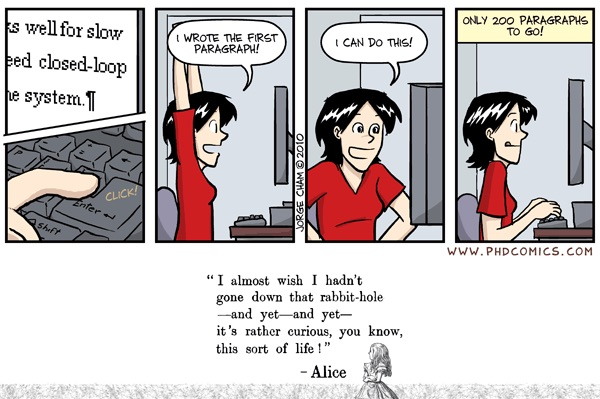
\includegraphics[width=0.9\textwidth]{./images/phd022410s.jpg}
    \caption{Here is a comic from \href{http://phdcomics.com/comics/archive.php?comicid=1285}{PhDComics}. (The previous word is also a clickable link! But if you click it, don't fall down the rabbit hole reading comics rather than writing your essay!). If you get stuck procrastinating, read this article as an antidote: \href{https://www.waitbutwhy.com/2013/10/why-procrastinators-procrastinate.html}{Why procrastinators procrastinate}. }
    \label{fig:example}
\end{figure}


\section{\LaTeX\ Mathematics Examples}
 
These math examples are courtesy of Prof Tony Roberts from The University of Adelaide. See \href{http://www.maths.adelaide.edu.au/anthony.roberts/LaTeX/Src/maths.tex}{here}.
 
\subsection{Delimiters}

See how the delimiters are of reasonable size in these examples
\[
	\left(a+b\right)\left[1-\frac{b}{a+b}\right]=a\,,
\]
\[
	\sqrt{|xy|}\leq\left|\frac{x+y}{2}\right|,
\]
even when there is no matching delimiter
\[
	\int_a^bu\frac{d^2v}{dx^2}\,dx
	=\left.u\frac{dv}{dx}\right|_a^b
	-\int_a^b\frac{du}{dx}\frac{dv}{dx}\,dx.
\]






\subsection{Spacing}

Differentials often need a bit of help with their spacing as in
\[
	\iint xy^2\,dx\,dy 
	=\frac{1}{6}x^2y^3,
\]
whereas vector problems often lead to statements such as
\[
	u=\frac{-y}{x^2+y^2}\,,\quad
	v=\frac{x}{x^2+y^2}\,,\quad\text{and}\quad
	w=0\,.
\]
Occasionally one gets horrible line breaks when using a list in mathematics such as listing the first twelve primes  \(2,3,5,7,11,13,17,19,23,29,31,37\)\,.
In such cases, perhaps include \verb|\mathcode`\,="213B| inside the inline maths environment so that the list breaks: \(\mathcode`\,="213B 2,3,5,7,11,13,17,19,23,29,31,37\)\,.
Be discerning about when to do this as the spacing is different.






\subsection{Arrays}

Arrays of mathematics are typeset using one of the matrix environments as 
in
\[
	\begin{bmatrix}
		1 & x & 0 \\
		0 & 1 & -1
	\end{bmatrix}\begin{bmatrix}
		1  \\
		y  \\
		1
	\end{bmatrix}
	=\begin{bmatrix}
		1+xy  \\
		y-1
	\end{bmatrix}.
\]
Case statements use cases:
\[
	|x|=\begin{cases}
		x, & \text{if }x\geq 0\,,  \\
		-x, & \text{if }x< 0\,.
	\end{cases}
\]
Many arrays have lots of dots all over the place as in
\[
	\begin{matrix}
		-2 & 1 & 0 & 0 & \cdots & 0  \\
		1 & -2 & 1 & 0 & \cdots & 0  \\
		0 & 1 & -2 & 1 & \cdots & 0  \\
		0 & 0 & 1 & -2 & \ddots & \vdots \\
		\vdots & \vdots & \vdots & \ddots & \ddots & 1  \\
		0 & 0 & 0 & \cdots & 1 & -2
	\end{matrix}
\]






\subsection{Equation arrays}

In the flow of a fluid film we may report
\begin{eqnarray}
	u_\alpha & = & \epsilon^2 \kappa_{xxx} 
	\left( y-\frac{1}{2}y^2 \right),
	\label{equ}  \\
	v & = & \epsilon^3 \kappa_{xxx} y\,,
	\label{eqv}  \\
	p & = & \epsilon \kappa_{xx}\,.
	\label{eqp}
\end{eqnarray}
Alternatively, the curl of a vector field $(u,v,w)$ may be written 
with only one equation number:
\begin{eqnarray}
	\omega_1 & = &
	\frac{\partial w}{\partial y}-\frac{\partial v}{\partial z}\,,
	\nonumber  \\
	\omega_2 & = & 
	\frac{\partial u}{\partial z}-\frac{\partial w}{\partial x}\,,
	\label{eqcurl}  \\
	\omega_3 & = & 
	\frac{\partial v}{\partial x}-\frac{\partial u}{\partial y}\,.
	\nonumber
\end{eqnarray}
Whereas a derivation may look like
\begin{eqnarray*}
	(p\wedge q)\vee(p\wedge\neg q) & = & p\wedge(q\vee\neg q)
	\quad\text{by distributive law}  \\
	 & = & p\wedge T \quad\text{by excluded middle}  \\
	 & = & p \quad\text{by identity}
\end{eqnarray*}






\subsection{Functions}

Observe that trigonometric and other elementary functions are typeset 
properly, even to the extent of providing a thin space if followed by 
a single letter argument:
\[
	\exp(i\theta)=\cos\theta +i\sin\theta\,,\quad
	\sinh(\log x)=\frac{1}{2}\left( x-\frac{1}{x} \right).
\]
With sub- and super-scripts placed properly on more complicated 
functions,
\[
	\lim_{q\to\infty}\|f(x)\|_q 
	=\max_{x}|f(x)|,
\]
and large operators, such as integrals and
\begin{eqnarray*}
	e^x & = & \sum_{n=0}^\infty \frac{x^n}{n!}
	\quad\text{where }n!=\prod_{i=1}^n i\,,  \\
	\overline{U_\alpha} & = & \bigcap_\alpha U_\alpha\,.
\end{eqnarray*}
In inline mathematics the scripts are correctly placed to the side in 
order to conserve vertical space, as in
\(
	1/(1-x)=\sum_{n=0}^\infty x^n.
\)






\subsection{Accents}

Mathematical accents are performed by a short command with one 
argument, such as
\[
	\tilde f(\omega)=\frac{1}{2\pi}
	\int_{-\infty}^\infty f(x)e^{-i\omega x}\,dx\,,
\]
or
\[
	\dot{\vec \omega}=\vec r\times\vec I\,.
\]





\subsection{Command definition}

\newcommand{\Ai}{\operatorname{Ai}} 
The Airy function, $\Ai(x)$, may be incorrectly defined as this 
integral
\[
	\Ai(x)=\int\exp(s^3+isx)\,ds\,.
\]

\newcommand{\D}[2]{\frac{\partial #2}{\partial #1}}
\newcommand{\DD}[2]{\frac{\partial^2 #2}{\partial #1^2}}
\renewcommand{\vec}[1]{\boldsymbol{#1}}

This vector identity serves nicely to illustrate two of the new 
commands:
\[
	\vec\nabla\times\vec q
	=\vec i\left(\D yw-\D zv\right)
	+\vec j\left(\D zu-\D xw\right)
	+\vec k\left(\D xv-\D yu\right).
\]

Recall that typesetting multi-line mathematics is an art normally too hard for computer recipes.  Nonetheless, if you need to be automatically flexible about multi-line mathematics, and you do not mind some rough typesetting, then perhaps invoke \verb|\parbox| to help as follows: 
% The \verb|breqn| package is not yet reliable enough for general use.
\newcommand{\parmath}[2][0.8\linewidth]{\parbox[t]{#1}%
    {\raggedright\linespread{1.2}\selectfont\(#2\)}}
\[
u_1=\parmath{ -2 \gamma  \epsilon^{2} s_{2}+\mu  \epsilon^{3} \big( \frac{3}{8} s_{2}+\frac{1}{8} s_{1} i\big)+\epsilon^{3} \big( -\frac{81}{32} s_{4} s_{2}^{2}-\frac{27}{16} s_{4} s_{2} s_{1} i+\frac{9}{32} s_{4} s_{1}^{2}+\frac{27}{32} s_{3} s_{2}^{2} i-\frac{9}{16} s_{3} s_{2} s_{1}-\frac{3}{32} s_{3} s_{1}^{2} i\big) +\int_a^b 1-2x+3x^2-4x^3\,dx }
\]
Also, sometimes use \verb|\parbox| to typeset multiline entries in tables.


\subsection{Theorems et al.}

\newtheorem{theorem}{Theorem}
\newtheorem{corollary}[theorem]{Corollary}
\newtheorem{lemma}[theorem]{Lemma}
\newtheorem{definition}[theorem]{Definition}

\begin{definition}[right-angled triangles] \label{def:tri}
A \emph{right-angled triangle} is a triangle \\ whose sides of length~\(a\), \(b\) and~\(c\), in some permutation of order, satisfies \(a^2+b^2=c^2\).
\end{definition}

\begin{lemma} 
The triangle with sides of length~\(3\), \(4\) and~\(5\) is right-angled.
\end{lemma}

This lemma follows from the Definition~\ref{def:tri} as \(3^2+4^2=9+16=25=5^2\).

\begin{theorem}[Pythagorean triplets] \label{thm:py}
Triangles with sides of length \(a=p^2-q^2\), \(b=2pq\) and \(c=p^2+q^2\) are right-angled triangles.
\end{theorem}

Prove this Theorem~\ref{thm:py} by the algebra \(a^2+b^2 =(p^2-q^2)^2+(2pq)^2
=p^4-2p^2q^2+q^4+4p^2q^2
=p^4+2p^2q^2+q^4
=(p^2+q^2)^2 =c^2\).


\section{Results}
 
\lipsum[43] % generic text; delete this and replace with your text

\subsection{These are the things that I learnt} 
 
\lipsum[44] % generic text; delete this and replace with your text

\section{Conclusion}
 
In conclusion, here are some more references \cite{Pincus2016,Hardy2016,Einstein1906,Turok1996}. 
 
\lipsum[53-55] % generic text; delete this and replace with your text

% You can add/remove chapters

\section{Acknowledgements}

Acknowledgements aren't mandatory, but it is always nice to thank people that helped you with your project (both, directly and indirectly).

%%%%%%%%%%%%%%%%%%%%%%%%%%%%%%%%%%%%%%%
%% THE REFERENCES - EDIT THESE FILES %%
%%%%%%%%%%%%%%%%%%%%%%%%%%%%%%%%%%%%%%%
\bibliographystyle{style_files/utphys}
\bibliography{references}

%%%%%%%%%%%%%%%%%%%%%%%%%%%%%%%%%%%%%%%
%% THE APPENDICES - EDIT THESE FILES %%
%%%%%%%%%%%%%%%%%%%%%%%%%%%%%%%%%%%%%%%
\begin{subappendices} % DO NOT EDIT THIS LINE
\renewcommand\thesection{\Alph{section}} % DO NOT EDIT THIS LINE

\section{One appendix}

\lipsum[5] % generic text; delete this and replace with your text

\subsection{And a subappendix}

\lipsum[6] % generic text; delete this and replace with your text

\section{Another appendix}

\lipsum[33] % generic text; delete this and replace with your text

% You can add/remove appendices

\end{subappendices} % DO NOT EDIT THIS LINE

% \cleardoublepage % makes sure there is an even number of pages for the book compilation (ignore this)

\end{document}